\section{Results}
\label{sec:results}

\subsection{Parameter settings}

In all of the following results, we use a suite size of 1200 (that is, 1200
independent simulations with different random number seeds for \textit{each}
combination of distinct independent variable values) and run each simulation
for 400 iterations. We set $V_N=20$ voters, $C_N=3$ candidates, $I_N=3$ issues,
$p_e=.2$ edge probability, and $E=50$ for eight consecutive elections in the
400 iteration time period.

\subsection{Multiple chasers impede one another}

Using the default voting algorithm distribution ($\frac{1}{3}$ rational,
$\frac{1}{3}$ party, $\frac{1}{6}$ F\&F1, $\frac{1}{6}$ F\&F2)
When only one of three candidates is chasing votes, it reaches its ``sweet
spot'' early on, and quickly encounters diminishing returns to further chasing.
When two candidates are chasing, they take longer to reach their equilibrium.
(See Figure~\ref{one_vs_two_chasers}.) We speculate that this is because the
chasers are interfering with one another as they court voters in opinion space,
dampening the gains of their rival by moving into regions that might have been
unspoken for.

\begin{figure}[ht]
\centering
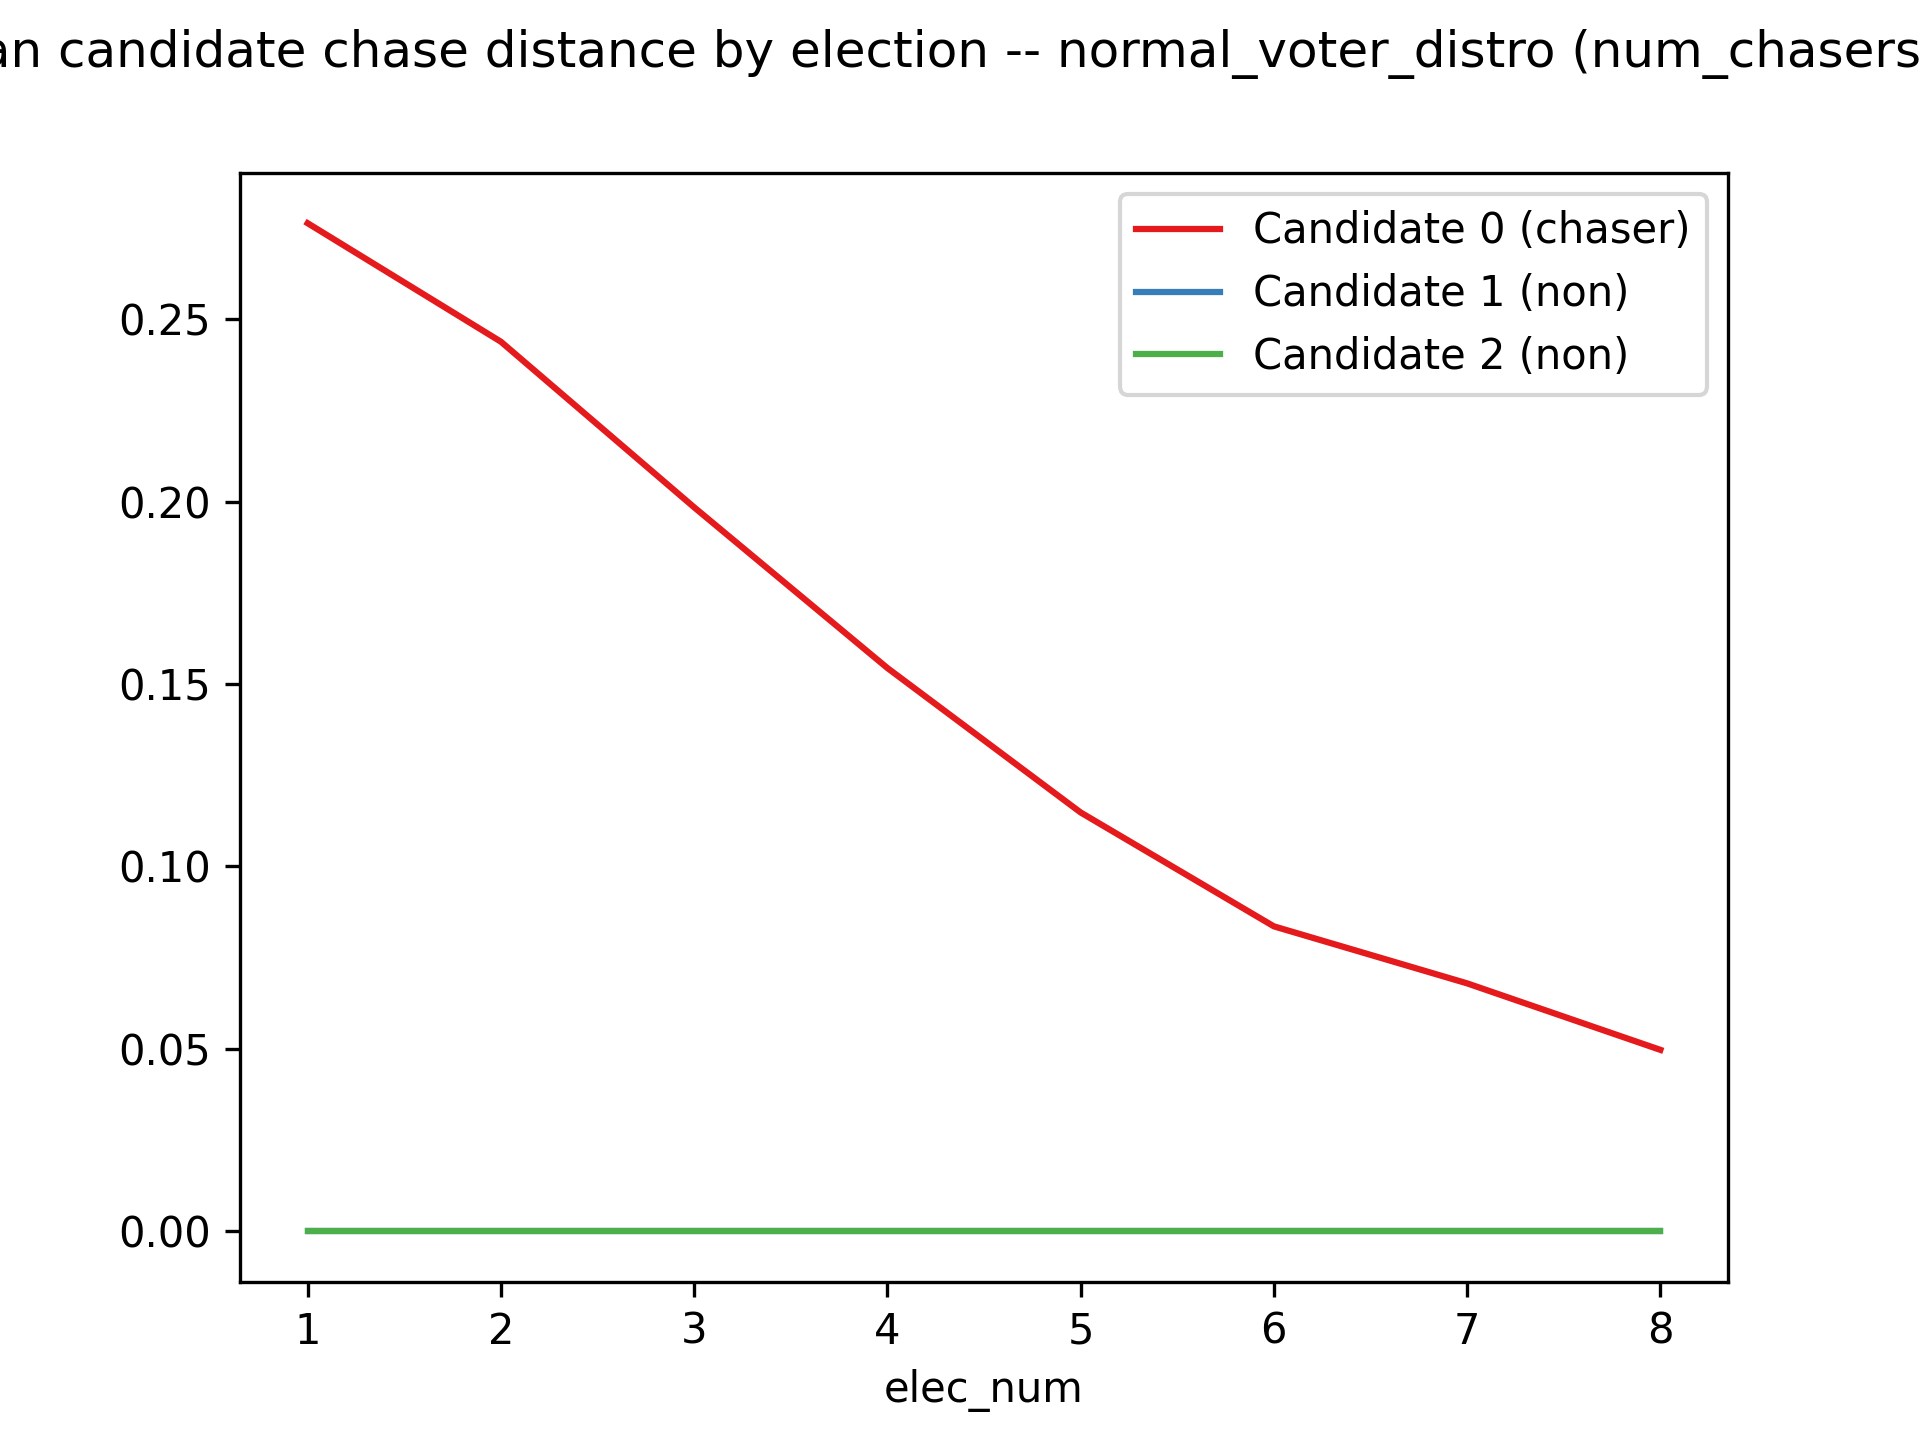
\includegraphics[width=0.45\textwidth]{assets/one_chaser_maxes_out_soon.png}
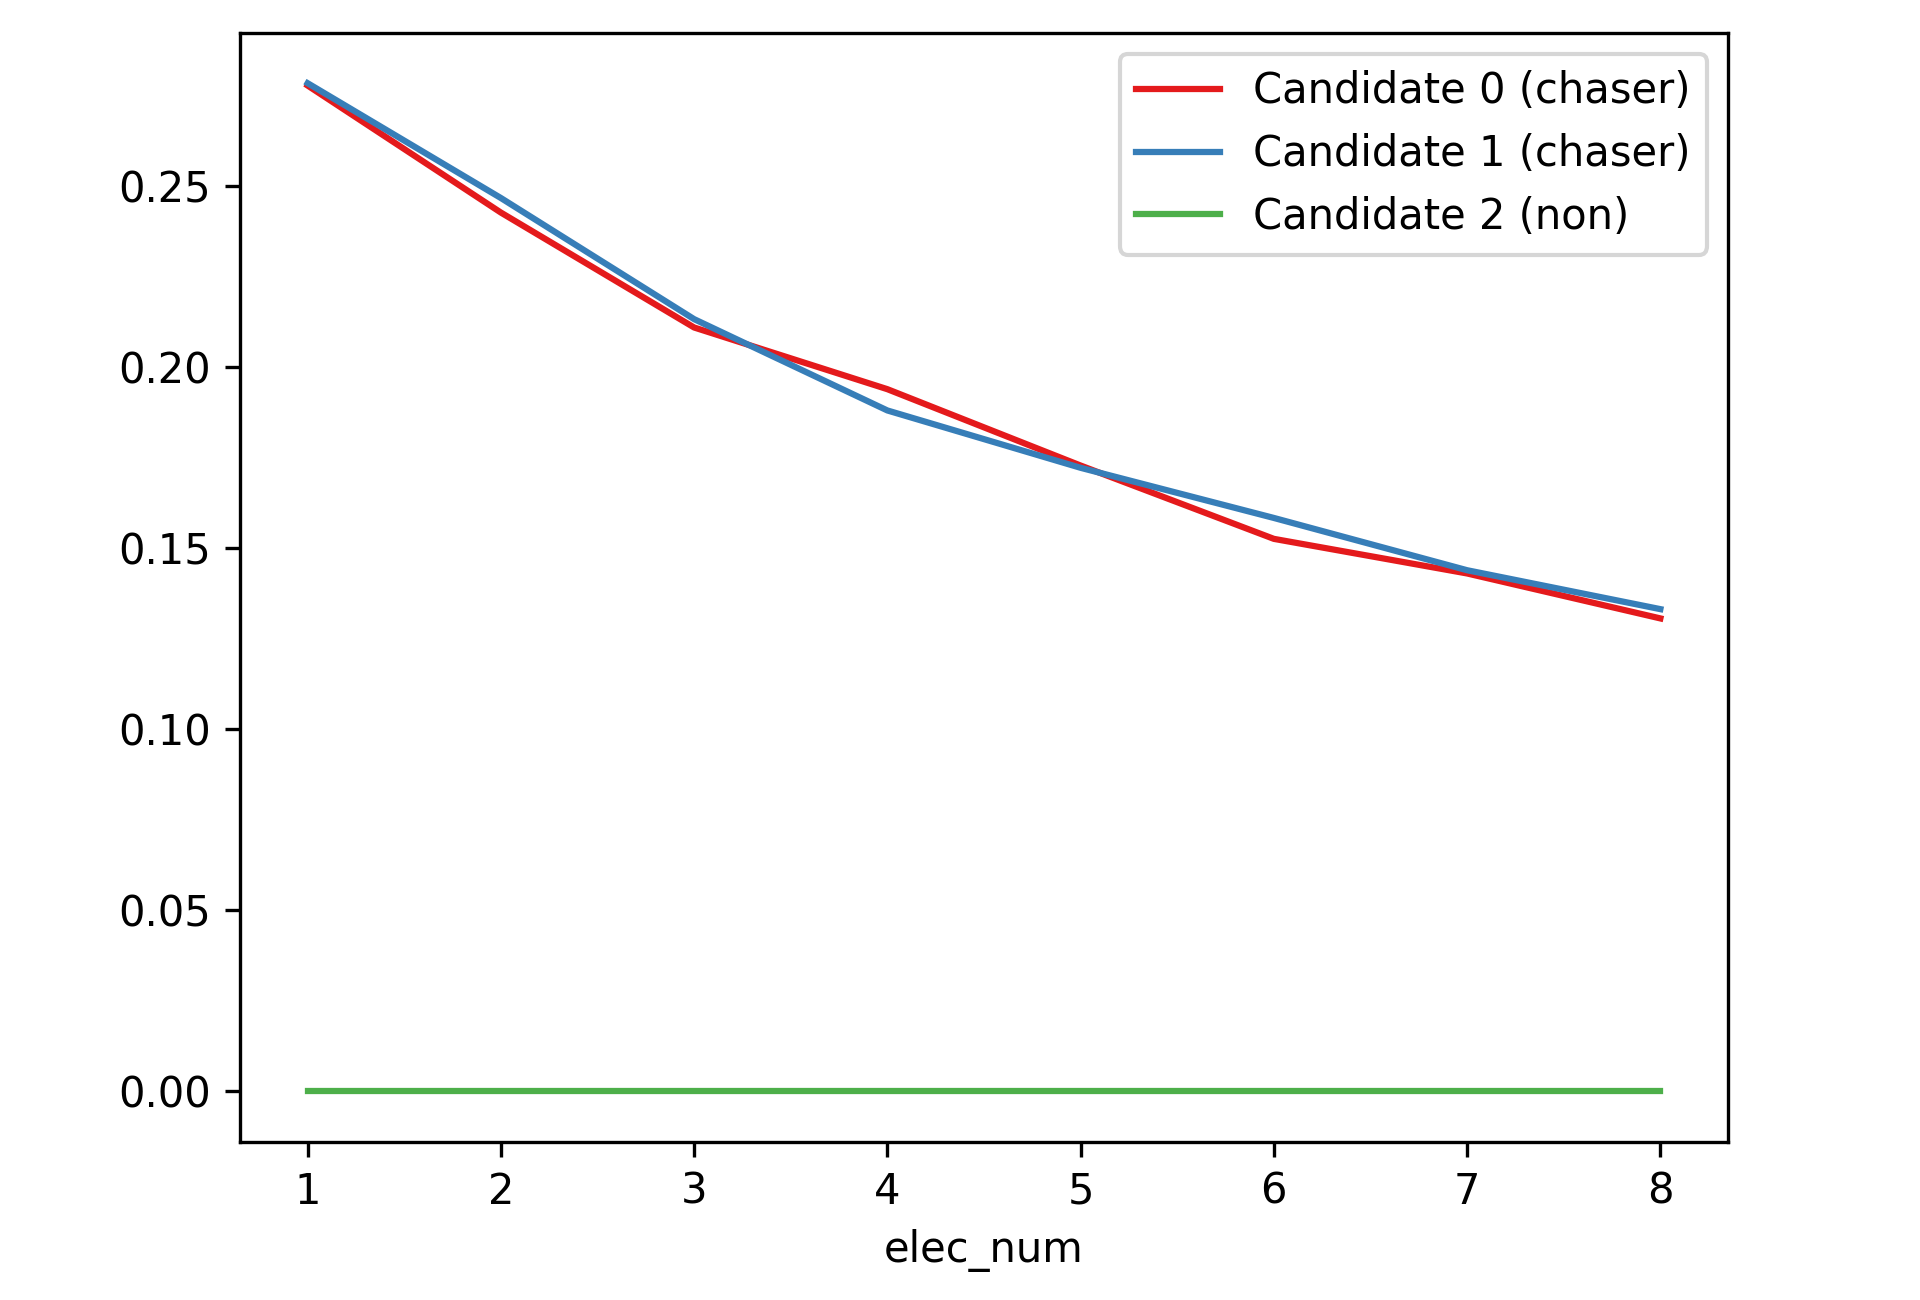
\includegraphics[width=0.45\textwidth]{assets/two_chasers_max_out_later.png}
\caption{A single chasing candidate maxes out its gains more quickly than two
competing chasers do.}
\label{one_vs_two_chasers}
\end{figure}

% Default voting makeup:
%    - Rationality: doesn't matter how many chasers. Rationality sucks.
%    - * Winning: one chaser gets incredible benefit, if there's only one.
%    This will be plot 4a and 4b
% No rational voters:
%    - Rationality: doesn't matter how many chasers. Rationality sucks.
%    - * Winning: chaser doesn't get any appreciable benefit.
%    This will be plot 5
% No FF voters:
%    - Rationality: doesn't matter how many chasers. Rationality overall better.
%    - * Winning: one chaser gets incredible benefit, if there's only one.
% All party voters:
%    - Rationality: Rationality REALLY sucks. Each additional chaser makes this
%    noticeably worse (though not stat sig).
%    - * Winning: chaser doesn't get any appreciable benefit.
% All rational voters:
%    - Rationality: Rationality uniformly perfect.
%    - * Winning: one chaser gets incredible benefit, if there's only one.
%      * Now if there are two, they both get incredible benefit.
%    This will be plot 6a and 6b  (contrast with 4a and 4b)
% All FF voters:
%    - Rationality: doesn't matter how many chasers. Rationality really sucks.
%    - * Winning: chaser doesn't get any appreciable benefit.

% Question for us to figure out: why, if default voter alg, only one chaser
% gets any benefit (two chasers cancel each others' benefits out stat sig) but
% if all voters are rational, then two chasers both benefit.


% Some preliminary findings and questions:

% chasing does pay off if lots of rational voters.
% chasing does not pay off if lots of party voters.
% Is there a correlation between how much each candidate chased (total sum of Euclidean distances of all chase actions) and how often they won

% does chasing ever hurt a candidate? hypothesis: if voters easily switch
% parties, and a candidate "overchases" and outruns their base, they will lose
% their base and this will hurt them. Can we reproduce this?

% Is there a correlation between how much the voting population is drifting and how likely the election at that time is to be rational?




